\documentclass[14]{article}
\usepackage{arxiv}
\usepackage[english, russian]{babel}
\usepackage[T1]{fontenc}
\usepackage{url}
\usepackage{booktabs}
\usepackage{amsfonts}
\usepackage{nicefrac}
\usepackage{microtype}
\usepackage{multicol}
\usepackage{lipsum}
\usepackage{graphicx}
\usepackage{natbib}
\usepackage{doi}
\usepackage[utf8]{inputenc}
\usepackage{amsmath}
\usepackage{mathtools}
\usepackage{algpseudocode}
\usepackage{algorithm2e}
\usepackage{ dsfont }
\usepackage{setspace}


\title{Дистилляция знаний в глубоких сетях}

\author{ Михаил Олейник \\ 
  МФТИ \\
  \texttt{oleinik.ms@phystech.edu} \\
  \And
  М. Горпинич \\ 
  МФТИ \\
  \texttt{gorpinich.m@phystech.edu} \\
  \And
  О. Ю. Бахтеев \\ 
  МФТИ \\ 
  \texttt{bakhteev@phystech.edu} \\
}
\date{}

\renewcommand{\undertitle}{}
\renewcommand{\headeright}{}
\renewcommand{\shorttitle}{Дистилляция знаний в глубоких сетях}

\hypersetup{
pdftitle={Дистилляция знаний в глубоких сетях},
pdfauthor={Михаил Олейник},
pdfkeywords={дистилляция модели \and байесовский вывод \and глубокое обучение \and вариационная оптимизация},
}

\begin{document}
\maketitle

\begin{abstract}
  Дистилляция знаний позволяет повысить качество модели, называемой учеником, не увеличивая её число параметров,
  а используя модель большего размера, называемой учителем.
  Однако, в случае разных архитектур и несовпадения количества слоев у учителя и ученика, распространённые методы не применимы.
  Одним из подходов, который позволяет решать задачу для разных архитектур, является максимизация взаимной информации.
  Мы предлагаем улучшение этого подхода, которое позволит проводить дистилляцию и для моделей с разным количеством слоёв.
  Мы сравниваем наш метод с остальными с помощью вычиcлительного эксперимента.
  Также проводим анализ гиперпараметров и выводим ограничения на них, при которых достигается наибольшее качество.
\end{abstract}

\keywords{дистилляция модели \and байесовский вывод \and глубокое обучение \and вариационная оптимизация}


\section{Введение}
Глубокие нейронные достигли больших успехов в задачах машинного зрения, обработки естественного языка и других.
Однако, лучшие результаты достигают модели с большим количеством параметров,
из-за этого их трудно встроить в системы с небольшими вычислительными мощностями, например, мобильные телефоны.
Если подобрать размер модели под целевую платформу, уменьшив количество параметров, то сильно потеряем и в качестве.

Одним из подходов, которые позволяют не теряя сильно в качестве, получить модель с меньшим количеством параметров, является дистилляция знаний.
Этот подход использует большую предобученную на необходимой задаче модель, называемую учителем,
данные о слоях которой переносятся определенным образом в модель меньшего размера, называемую учеником.
Перенос чаще всего выражается в дополнительном слагаемом в функции потерь ученика.

Так, в работе \cite{hinton2015distilling} предлагается переносить знания с последнего слоя модели.
К недостаткам этого метода можно отнести то, что мы игнорируем информацию из остальных слоев учителя, а она может быть ценной.
В работах ...

Однако, большинство подходов либо неэффективно работают, либо не могут быть применимы к случаям, когда модели имеют разное количество слоёв или разную архитектуру.
Также возникают сложности в случае, когда количество параметров в слое учителя сильно больше,
чем в соответствующем слое ученика, как показано в работе \cite{mirzadeh2020improved}.

Больший интерес представляют подходы, которые можно применить, если учитель и ученик имеют разные архитектуры.
В работе \cite{passalis2020heterogeneous} моделируется информационный поток в учителе, который имитирует ученик.
В работе \cite{Ahn_2019_CVPR} используется максимизация взаимной информации между парами соответствующих слоёв.
В основе этого метода используется вариационный подход \cite{barber2004algorithm}.
Наша работа предлагает улучшение данного метода, давая возможность проведения дистилляции при разном количестве слоев у учителя и ученика.
Также мы проводим анализ гиперпараметров алгоритма, на примере работы \cite{gorpinich2022gradient}.

\section{Постановка задачи}

Дан датасет для задачи многоклассовой классификации, с количеством классов $K$:

$$\mathfrak{D}  = \{(\bold{x}_i, y_i)\}_{i=1}^{m},\; \bold{x}_i \in \mathbb{R}^n,\; y_i \in \mathbb{Y}  = \{1, \dots, K\},$$

Датасет разбит на обучающую и тестовую выборку: $\mathfrak{D} = \mathfrak{D}_\text{train} \bigsqcup \mathfrak{D}_\text{test}$.

Дана модель учителя $\bold{f}$, обученная на $\mathfrak{D}_\text{train}$.
Дана модель ученика $\bold{g}$, которую предстоит обучить.

Пусть $T$ --- количество слоев в модели учителя, $S$ --- количество слоев в модели ученика.
Обозначим как $t_i$ и $s_j$ --- активации в $i$-м слое учителя и в $j$-м слое ученика, соответственно.

Функцию потерь ученика представим как:

$$
  \mathcal{L} = \beta \mathcal{L}_\text{task} + (1 - \beta){\sum_{i, j=1}^{T, S}\lambda_{i, j}I(t_{i}, s_{j})},
$$
\noindent
где $\mathcal{L}_\text{task}$ --- функция потерь для решения задачи классификации,
$I(t_{i}, s_{j})$ --- взаимная информация, $\beta$ и $\lambda_{i, j}$ --- гиперпараметры.

\section{Вычислительный эксперимент}

\subsection{Базовый эксперимент}

Был проведён эксперимент с использованием датасета CIFAR10. В качестве модели учителя была выбрана модель \textbf{ResNet-18},
в качестве учеников --- две свёрточные нейронные сети, под кодовыми названиями \textbf{tiny} и \textbf{very\_tiny}.

Цель --- сравнение качества учеников с и без дистилляции Хинтона, а также зависимость качества
дистиллированных моделей от гиперпараметров $\beta$ и $T$.

\begin{figure}[h]
  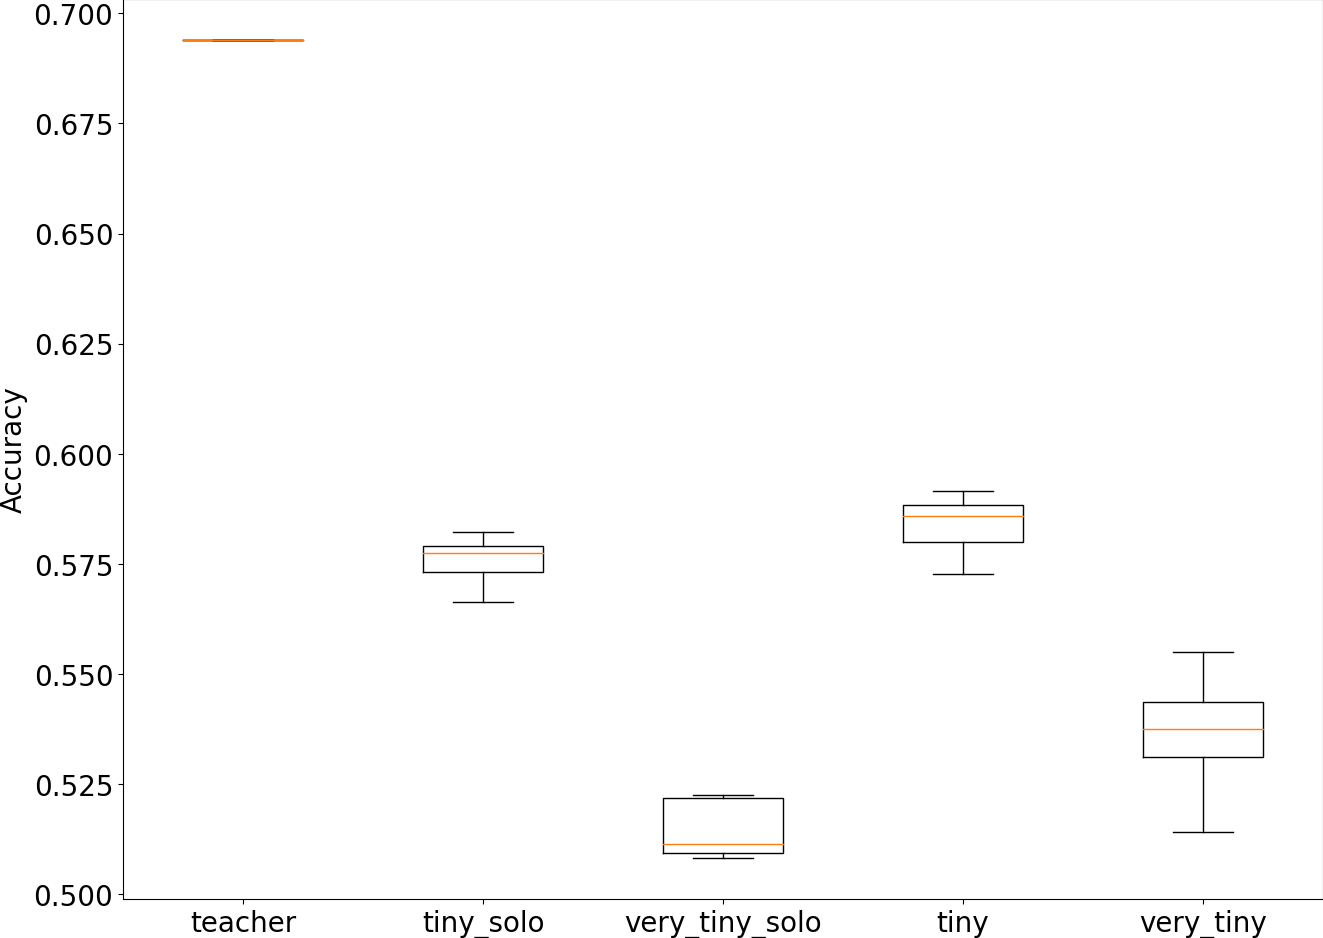
\includegraphics[width=9cm]{../figures/box_hinton_model_accuracy.png}
  \centering
  \caption{Сравнение качества моделей.}
\end{figure}

\begin{figure}[h]
  \begin{multicols}{2}
    \hfill
    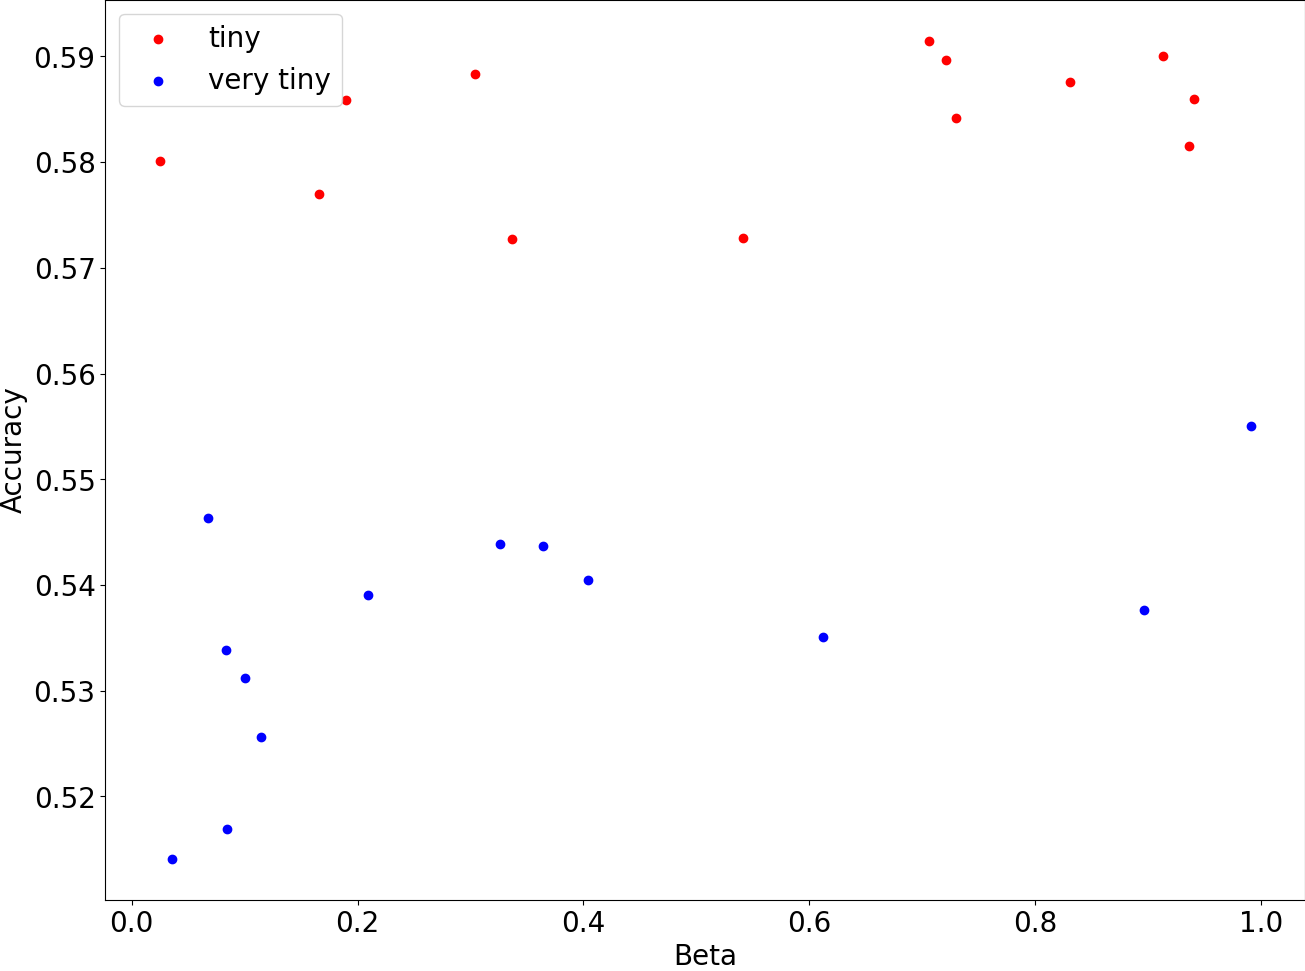
\includegraphics[width=0.5\textwidth]{../figures/scatter_hinton_beta_acc.png}
    \hfill
    \caption{Зависимость качества от параметра $\beta$.}
    \hfill
    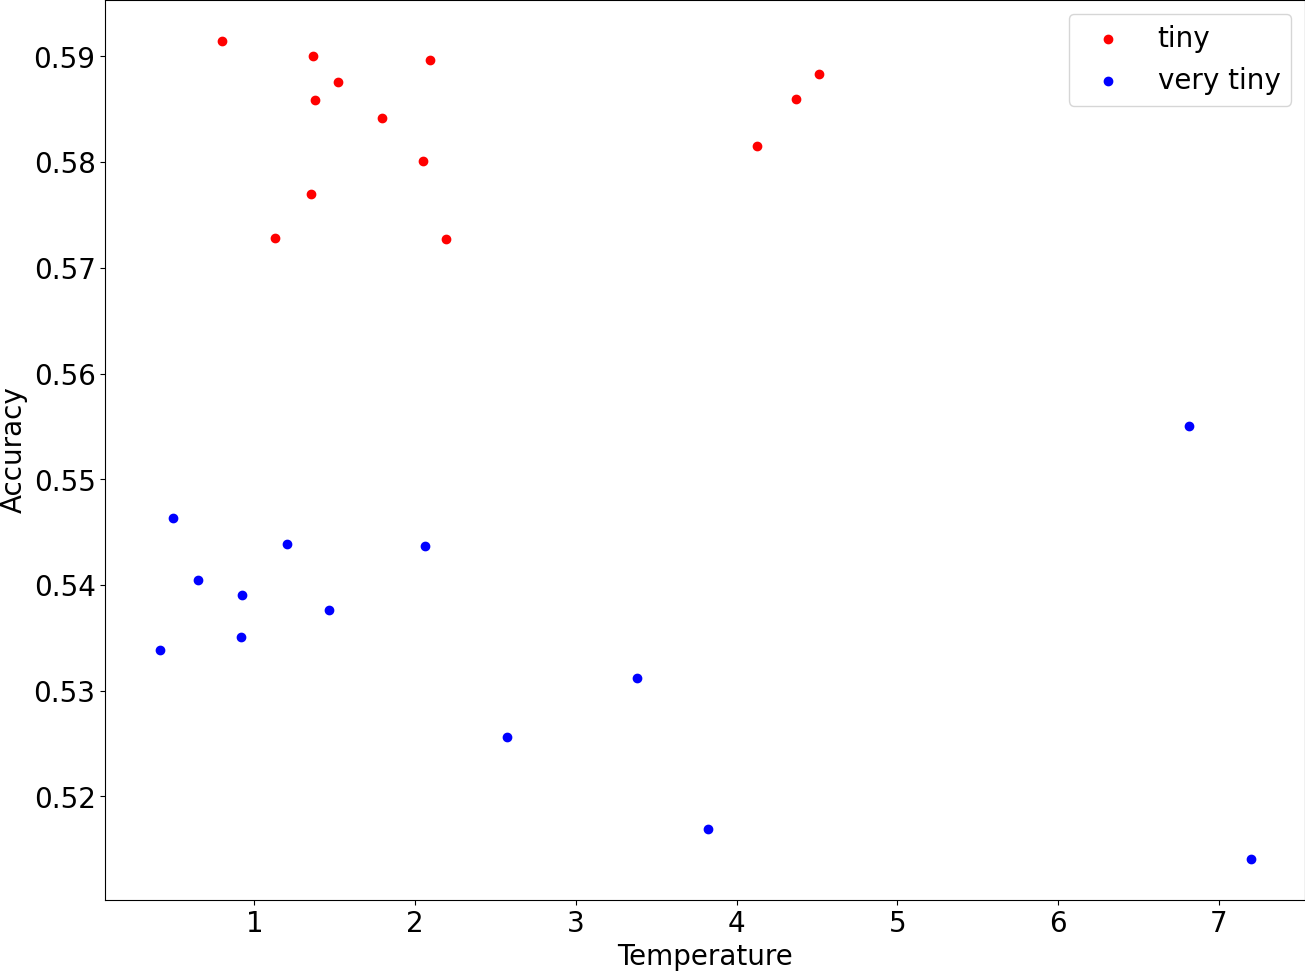
\includegraphics[width=0.5\textwidth]{../figures/scatter_hinton_temp_acc.png}
    \hfill
    \caption{Зависимость качества от параметра $T$.}
  \end{multicols}
\end{figure}

\subsection{Основной эксперимент}




\newpage
\bibliographystyle{unsrt}
\bibliography{references.bib}

\end{document}